% Macros de estilo
% Definimos nuevos comandos para facilitar la uniformidad de estilos.
% Ayudará, por supuesto, crear atajos de teclado que los introduzcan, o
% tener un editor que ayude con el autocompletado.

% Palabras en inglés: \ingles
% Definimos tanto el estilo general como el idioma. Lo del idioma es necesario
% porque el paquete de idioma define muchas cuestiones. Ver la documentación
% del paquete Polyglossia o del paquete Babel.
% Usamos cursivas (_italics_) para los extranjerismos.
\newcommand{\ingles}[1]{\textit{\texten{#1}}}


% Nombres propios: \nombre{}
% Ya sean personas o instituciones. Nombres no genéricos. Títulos de libros o documentos no.
% Usamos una fuente _sans serif_.
\newcommand{\nombre}[1]{\textsf{#1}}

% Programas y comandos: \programa{}
% Usamos una fuente monoespaciada.
\newcommand{\programa}[1]{\texttt{#1}}


% Atajo para una nota de cosas pendientes (dependiente del paquete
% todonotes). Lo usamos como 'inline' porque en los márgenes hay poco
% espacio y no se pueden leer. 
% Las notas de tipo 'inline' pueden usarse en _captions_, mientras que
% las normales no.
% El atajo queda entonces como \td{}
%\def\td{\todo[inline]}
\newcommand{\td}[1]{\todo[inline]{#1}{}}



%\begin{figure}[hbtp]
%\centering
%\includegraphics[width=0.4\linewidth]{dummy}
%\caption[]{\td{Cita}}
%\label{fig:}
%\end{figure}


% Anchos predefinidos para las imágenes.
\def\imagenchica{5cm}
\def\imagenmedia{10cm}
\def\imagengrande{15cm}
% Se pueden usar así: 
%\begin{figure}[hbtp]
%    \centering
%    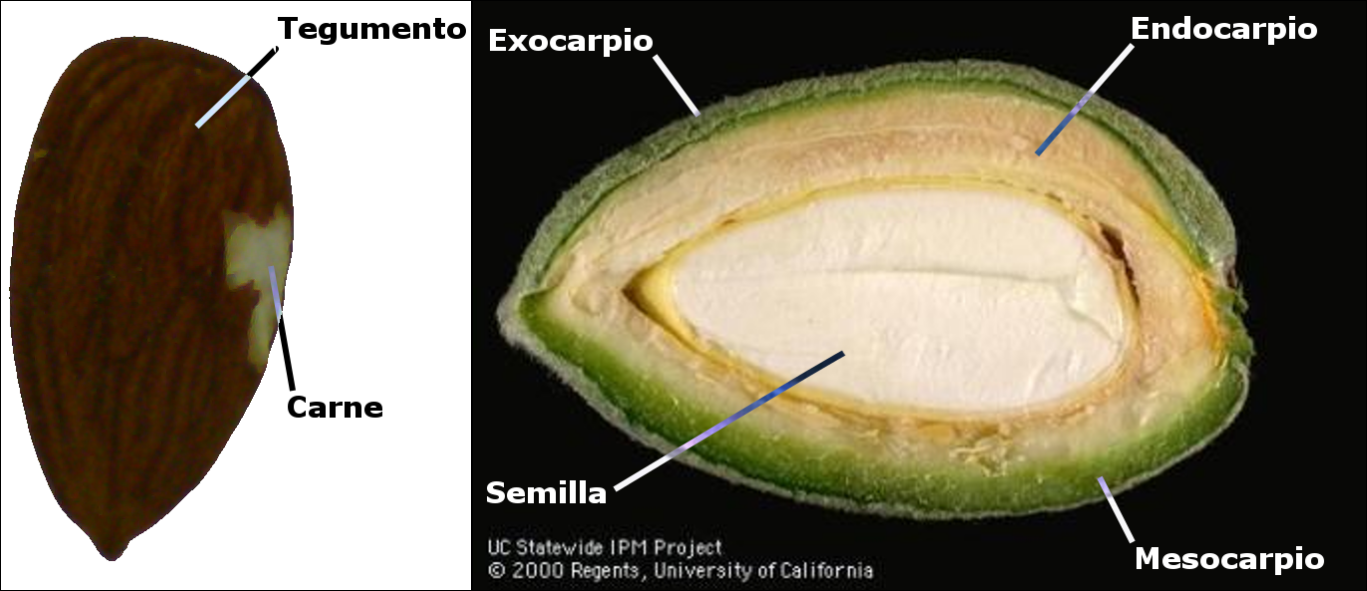
\includegraphics[width=\imagengrande]{almendra_partes_1_2}
%    \caption[Partes de una almendra]{partes de una almendra. Izquierda: semilla; derecha: corte de un fruto completo.~\autocite[][]{imagenes:interioralmendra}}
%    \label{fig:partesalmendra}
%\end{figure}


% Macro para citar. ~ es un espacio que no se puede separar. Esto es, separa dos
% palabras pero hace que estas no puedan separarse en distintos renglones, por
% ejemplo.
% https://tex.stackexchange.com/questions/15547/when-should-i-use-non-breaking-space
\newcommand{\citar}[1]{~\autocite{#1}}
% Lamentablemente no me funciona el autocompletado de citas en TeXstudio si uso
% un comando personalizado, así que mejor poner \autocite{} a mano.